% Project 1 extended abstract (CCN two-page template from Moodle).
% Every number in this file comes from results/v2 (collapse.json, mechanism.json,
% choice_profiles.json, formation/*.json); see README.txt for the commands.

\documentclass[10pt,letterpaper]{article}

\usepackage{ccn}
\usepackage{pslatex}
\usepackage{apacite}
\usepackage{graphicx}
\usepackage{caption}
\usepackage{natbib}
\usepackage{float}

\usepackage{hyperref}       % hyperlinks
\usepackage{url}            % simple URL typesetting
\usepackage{booktabs}       % professional-quality tables
\usepackage{amsfonts}       % blackboard math symbols
\usepackage{nicefrac}       % compact symbols for 1/2, etc.
\usepackage{microtype}      % microtypography
\usepackage{xcolor}         % colors
\usepackage{amsmath}
\usepackage{amssymb}
\usepackage{mathtools}
\usepackage{amsthm}
\usepackage{svg}
\usepackage{pdfpages}
\usepackage[labelfont=bf, margin=0.8cm, font=sf]{caption}

% NeurIPS checklist answer macros (from neurips_2024.sty, which can't be loaded with ccn.sty)
\newcommand{\answerYes}[1][]{\textcolor{blue}{[Yes] #1}}
\newcommand{\answerNo}[1][]{\textcolor{orange}{[No] #1}}
\newcommand{\answerNA}[1][]{\textcolor{gray}{[NA] #1}}

\title{Collapse Without Circuit Damage: Recursive Training Corrupts\\a Choice Made Outside the Induction Circuit}

% Authors in alphabetical order of surname; student numbers in brackets.
\author{{\large \bf Shervaan Govinder (2556996)} \\ University of the Witwatersrand, 1 Jan Smuts Ave,\\ Braamfontein, Johannesburg, 2000, South Africa
  \AND {\large \bf Jaishil Patel (2602867)} \\ University of the Witwatersrand, 1 Jan Smuts Ave,\\ Braamfontein, Johannesburg, 2000, South Africa
  \AND {\large \bf Kovendan Jason Raman (2566527)} \\ University of the Witwatersrand, 1 Jan Smuts Ave,\\ Braamfontein, Johannesburg, 2000, South Africa}


\begin{document}

\maketitle
\phantom{.}
\newpage
\phantom{.}
\newpage
\section{Abstract}
{
\bf
\looseness=-1
We ask how model collapse affects in-context learning (ICL) and the induction circuit that implements it. We train two-layer transformers on an adaptation of Singh et al.'s symbol--label task and retrain them for 6--8 generations on their predecessor's outputs. When the model writes only the query's label, nothing collapses. When it also chooses a next symbol, the choice collapses (KL on real data 0.10$\to$0.56 nats in two seeds) while query accuracy stays $\geq$0.999, because the choice is computed outside the circuit: the key path that carries 99\% of the previous-token head's effect on the query label leaves it unchanged. An exact split of the KL separates \emph{leakage} out of the context, which filtering and longer training reduce, from \emph{misallocation} within it, which neither reduces. At temperature 0.7 the collapse is mostly sampling arithmetic, and models that write their own contexts still copy correctly. Collapse corrupts a choice made outside the induction circuit, not the circuit itself.
}
\begin{quote}
\small
\textbf{Keywords:}
model collapse; induction heads; mechanistic interpretability
\end{quote}

\section{Introduction} \label{Intro}
\looseness=-1
Much of ICL is carried by \emph{induction heads}: at a repeated token $A$, a layer-1 head attends to whatever followed the earlier $A$ and copies it, finding that position through a key written by a layer-0 \emph{previous-token head} \citep{elhage2021mathematical,olsson2022context}. \citet{singh2024needs} dissected how this circuit forms on arbitrary but consistent symbol--label pairs. \emph{Model collapse} is the degradation of models trained recursively on their predecessors' outputs: errors compound and the tails of the distribution vanish \citep{shumailov2023curse,shumailov2024collapse}, unless real data is kept \citep{gerstgrasser2024inevitable}. Its effect on the \emph{mechanisms} inside a model is unknown. We track both the circuit and the collapsing behaviour with causal interventions \citep{conmy2023automated} and data deletions.

\begin{figure*}[t]
  \centering
  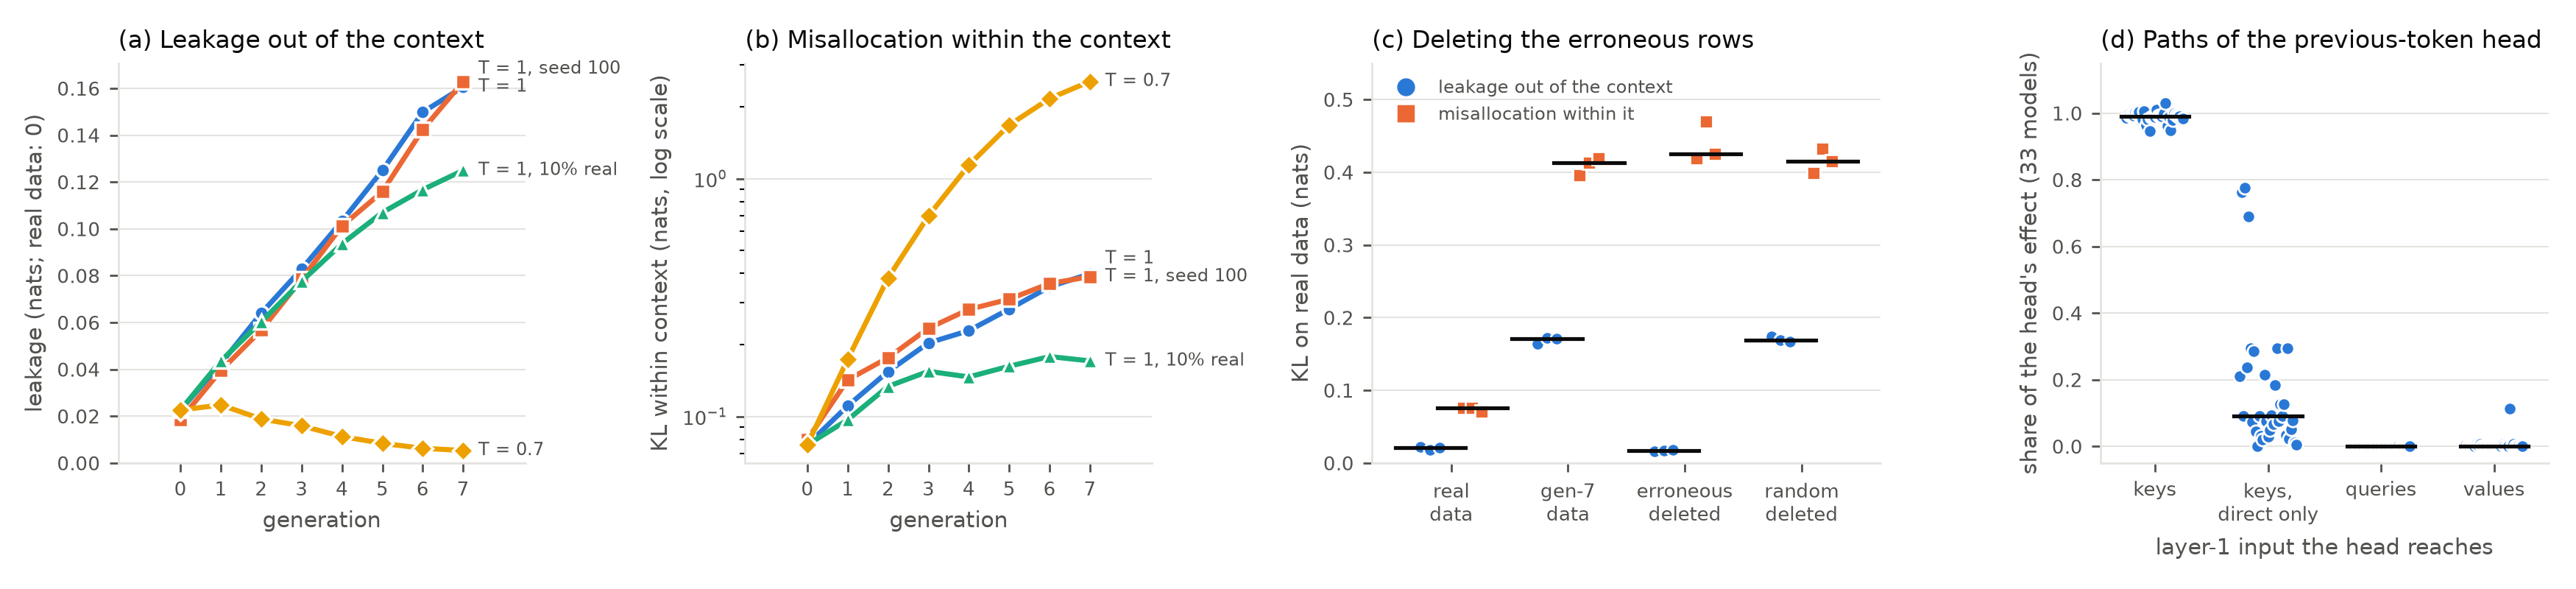
\includegraphics[width=\textwidth]{images/fig_main.png}
  \vspace{-14pt}
  \caption{\looseness=-1 (a) Leakage on real data rises at $T{=}1$ and falls at $T{=}0.7$. (b) Misallocation (log scale) rises in every chain; 10\% real data caps it. (c) Deleting generation-7's contradicting rows restores leakage (blue) but not misallocation (orange); random deletion does neither (dots: seeds; bars: medians). (d) Share of the previous-token head's effect on the query label carried by each path into layer 1 (33 models of the first five chains): almost all reaches the keys, mostly via the layer-0 MLP.}
  \label{fig:main}
\end{figure*}

\section{Methods}
\looseness=-1
\textbf{Task and model.} We adapt Singh et al.'s task (Omniglot exemplars, two pairs, attention-only models) to tokens: 8 (symbol, label) pairs from 32 symbols and 8 labels, consistently paired within a sequence, then a query symbol from the context. With distinct symbols and a query-only loss our models stayed for 20{,}000 steps at the 0.325 accuracy that label counting reaches without induction. Longer training might escape this, but with 4 distinct symbols per sequence and a loss on every repeated symbol's label (no-induction ceiling 0.523) induction forms in every run. The model is a 2-layer transformer (4 heads, $d_\text{model}{=}64$, MLP 256, 103k parameters) trained with AdamW (learning rate $10^{-3}$ throughout, batch 256), chosen by a $3{\times}3$ sweep on validation loss, as validation accuracy saturates.

\textbf{Collapse pipeline.} Generation 0 trains on 200{,}000 real sequences, generation $g$ on 200{,}000 with fresh real contexts and answers \emph{sampled} at temperature $T$ by generation $g{-}1$. The \emph{base} variant writes the query label; the \emph{extended} variant also writes a next symbol, whose true probability is $q(s){=}c/8$ for a symbol in $c$ of the 8 slots, and its label. Real contexts make the base target a deterministic function of an uncorrupted input, unlike \citet{shumailov2024collapse}, so one chain lets the model write whole sequences. We ran the base variant for 6 generations (25{,}000 steps) and extended chains for 8 (8{,}000 steps): $T{=}1$, $T{=}0.7$ and 10\% real data with two seeds each, plus 25{,}000 steps, generated contexts and accumulated data \citep{gerstgrasser2024inevitable}.

\textbf{Measures.} Every reported measure, circuit tests included, uses one set of 10{,}000 held-out real sequences; a separate validation set (5{,}120) only times the phase change. As $q$ is exact, so is the KL of the next-symbol distribution $p$, which splits in two:
\begin{equation}
\mathrm{KL}(q\,\|\,p) = \underbrace{-\log(1-p_\text{out})}_{\text{leakage}} + \underbrace{\mathrm{KL}(q\,\|\,\tilde p)}_{\text{misallocation}},
\label{eq:split}
\end{equation}
where $p_\text{out}$ is the mass outside the context and $\tilde p$ is $p$ renormalised over it. A perfect learner turns sampling at $T$ into $p_g \propto p_0^{(1/T)^g}$, our null model. We use \emph{resample ablation} \citep{conmy2023automated} and \emph{path patching} \citep{goldowskydill2023localizing}, which resamples a layer-0 head only where layer 1 reads queries, keys or values, and score every intervention on both the query label and the next-symbol choice. In the spirit of \citet{chen2026mechanistic}, we retrain fresh models (3 seeds) on generation-7 data with or without its context-contradicting rows.

\section{Results}
\looseness=-1
\textbf{No collapse in the base variant.} Every generation reaches query accuracy 1.000 on real data, and errors in the generated labels fall from $4.5{\times}10^{-5}$ to $5{\times}10^{-6}$: models copy the context instead of learning the sampled errors (supplementary Table~\ref{tab:train}).

\textbf{The extended variant collapses only in its free choice.} Query and next-label accuracy on real data stay $\geq$0.997 in every generation of every chain, yet the next-symbol KL grows from 0.10 to 0.56 nats by generation 7 in both $T{=}1$ seeds (supplementary Table~\ref{tab:collapse}). Leakage adds about generation 0's own error each generation (Fig.~\ref{fig:main}a), but 70\% of the KL is misallocation among valid symbols (Fig.~\ref{fig:main}b). Training each generation 3$\times$ longer halves leakage (0.074 vs.\ 0.161 nats) but \emph{increases} misallocation (0.58 vs.\ 0.40 nats; one chain).

\textbf{Temperature decides which collapse occurs.} At $T{=}0.7$ leakage falls (0.023$\to$0.005 nats) while misallocation reaches 2.6--2.7 nats in two seeds and single-slot symbols nearly vanish (0.017--0.027; true 0.125). Through generation 4 the null model predicts this narrowing; afterwards the learner collapses \emph{less} than it (2.6 vs.\ 5.0 nats; supplementary Table~\ref{tab:null}). Keeping 10\% real data halves the KL and caps misallocation near 0.17--0.19 while leakage keeps rising; accumulating data keeps misallocation at its generation-0 level and leakage at 0.059 nats (supplementary Table~\ref{tab:revision}).

\textbf{Filtering removes the expected failure only.} Context-contradicting rows (14.5\% of generation-7 data) are the only source of out-of-context targets, so deleting them restores real-data leakage (0.016--0.018 vs.\ 0.018--0.023). Misallocation survives (0.42--0.47): it lives in rows that each look correct (Fig.~\ref{fig:main}c).

\textbf{Copying survives generated contexts.} A model that writes whole sequences keeps $\geq$99.5\% of repeated symbols paired with their label and real query accuracy $\geq$0.9997, while its free choices drift: the KL of its context symbols rises from 0.18 to 1.17 nats, and 8.3\% of its queries leave the context.

\textbf{The query circuit survives.} In all 78 models, resampling layer 1 drops query accuracy to near chance (0.13--0.14; chance 0.125) and layer 0 to 0.20--0.42, and previous-token and induction scores stay $\geq$0.89 and $\geq$0.96. Where one layer-0 head matters (70 models), its path into layer 1's \emph{keys} carries a median 99\% of its effect but the direct edge only 9\% (Fig.~\ref{fig:main}d): unlike \citet{singh2024needs}'s attention-only models, ours relay K-composition through the layer-0 MLP.

\textbf{The collapsing choice runs outside it.} Scored on the choice (72 models; supplementary Table~\ref{tab:choice}), patching the previous-token head into layer 1 changes the KL by at most 0.07 nats with real contexts (0.19 with generated ones), and the induction head matters no more than any other layer-1 head. Yet resampling layer 1 or layer 0 raises misallocation from 0.17 to 1.3--1.7 nats: the choice reads context symbols directly. At $T{=}0.7$, layer-1 attention stays near-uniform over the slots while the output sharpens.

\textbf{The objective sets when induction forms.} Removing the next-symbol target delays the phase change (validation accuracy $\geq$0.9) from 750--1{,}750 to 6{,}250--7{,}750 steps, while generation-7 data forms induction as fast as real data.

\section{Discussion}
\looseness=-1
With real contexts the query label is a deterministic function of the input, so a model that learns induction rejects sampled errors. This follows largely from the design, but a model that writes its own contexts still pairs and copies consistently. Collapse appears where the model has freedom, in a computation the circuit does not perform: matching choices to $c/8$ is counting, not copying. A model can pass every ICL accuracy test, and every circuit test built on them, while its generative distribution collapses.

Eq.~\ref{eq:split} separates two failures. Leakage, meaning impossible outputs, is approximation error: longer training shrinks it and a consistency filter removes it. Misallocation lives in rows that each look correct and grows with longer training, consistent with each model fitting its finite sample's noise, the statistical error of \citet{shumailov2024collapse}; only real data limits it. Temperature trades one failure for the other largely through sampling arithmetic, as biased sampling trades diversity for quality \citep{alemohammad2024mad}, and per-sample verification \citep{feng2025beyond} addresses only the visible half.

\textbf{Limitations.} Two seeds per temperature and for 10\% real data; one chain each for 25{,}000 steps, generated contexts and accumulation. Chains are short (8 generations), generation is confounded with seed, the deletion test covers one chain, and our task adapts rather than reproduces Singh et al.'s.

\section{Contribution Statements (Not in Page Limit)}
All three authors contributed equally. \textbf{Shervaan Govinder} implemented the transformer, the in-context learning task and the first collapse pipeline, ran the hyper-parameter sweeps and the seed-100 replication, and wrote the project's analysis tools. \textbf{Jaishil Patel} wrote the extended abstract, made the paper figures, and ran the embedding, attention, train-accuracy and leakage-recursion analyses. \textbf{Kovendan Jason Raman} implemented the recursive base variant, the real-data evaluation and the leakage/misallocation split, ran the collapse chains on the cluster, and carried out the path-patching, circuit-formation and data-deletion experiments. All authors designed the study, interpreted the results and edited the paper.

\section{Acknowledgements (Not in Page Limit)}
Computations were performed using High Performance Computing infrastructure provided by the Mathematical Sciences Support Unit at the University of the Witwatersrand.

\bibliographystyle{apacite}

\setlength{\bibleftmargin}{.125in}
\setlength{\bibindent}{-\bibleftmargin}

\bibliography{ccn_style}

% ---------------------------------------------------------------------------
% REQUIRED before submission (the project is not marked without the checklist):
%   1. NeurIPS 2024 checklist: paste the .tex from Moodle here and fill it in.
%   2. Wits Science Faculty AI Ethics Form.
% ---------------------------------------------------------------------------
\section*{NeurIPS Paper Checklist}
% NeurIPS 2024 paper checklist (template from Moodle, paper/NeurIPS_2024_checklist/).
% Instruction block removed as the template asks; questions and guidelines unchanged.

\begin{enumerate}

\item {\bf Claims}
    \item[] Question: Do the main claims made in the abstract and introduction accurately reflect the paper's contributions and scope?
    \item[] Answer: \answerYes{}
    \item[] Justification: The abstract and introduction claim that collapse in the extended variant affects only the free next-symbol choice, splits into leakage and misallocation with different causes, and leaves the induction circuit intact; these match the Results (Table~\ref{tab:collapse}, Fig.~\ref{fig:main}). The scope (two-layer transformers on a synthetic symbol--label task) is stated in Methods and Limitations.
    \item[] Guidelines:
    \begin{itemize}
        \item The answer NA means that the abstract and introduction do not include the claims made in the paper.
        \item The abstract and/or introduction should clearly state the claims made, including the contributions made in the paper and important assumptions and limitations. A No or NA answer to this question will not be perceived well by the reviewers. 
        \item The claims made should match theoretical and experimental results, and reflect how much the results can be expected to generalize to other settings. 
        \item It is fine to include aspirational goals as motivation as long as it is clear that these goals are not attained by the paper. 
    \end{itemize}

\item {\bf Limitations}
    \item[] Question: Does the paper discuss the limitations of the work performed by the authors?
    \item[] Answer: \answerYes{}
    \item[] Justification: The Limitations paragraph in the Discussion states the number of seeds per chain, the short chains, the confound between generation and seed, that the deletion test covers one chain, and that our task adapts Singh et al.'s; Methods states that keeping contexts real limits how far the base result generalises; supplementary Table~\ref{tab:fit} reports the weaker fit ($R^2{=}0.83$) where it occurs, and Table~\ref{tab:null} compares the $T{=}0.7$ chain with a null model of pure sampling.
    \item[] Guidelines:
    \begin{itemize}
        \item The answer NA means that the paper has no limitation while the answer No means that the paper has limitations, but those are not discussed in the paper. 
        \item The authors are encouraged to create a separate "Limitations" section in their paper.
        \item The paper should point out any strong assumptions and how robust the results are to violations of these assumptions (e.g., independence assumptions, noiseless settings, model well-specification, asymptotic approximations only holding locally). The authors should reflect on how these assumptions might be violated in practice and what the implications would be.
        \item The authors should reflect on the scope of the claims made, e.g., if the approach was only tested on a few datasets or with a few runs. In general, empirical results often depend on implicit assumptions, which should be articulated.
        \item The authors should reflect on the factors that influence the performance of the approach. For example, a facial recognition algorithm may perform poorly when image resolution is low or images are taken in low lighting. Or a speech-to-text system might not be used reliably to provide closed captions for online lectures because it fails to handle technical jargon.
        \item The authors should discuss the computational efficiency of the proposed algorithms and how they scale with dataset size.
        \item If applicable, the authors should discuss possible limitations of their approach to address problems of privacy and fairness.
        \item While the authors might fear that complete honesty about limitations might be used by reviewers as grounds for rejection, a worse outcome might be that reviewers discover limitations that aren't acknowledged in the paper. The authors should use their best judgment and recognize that individual actions in favor of transparency play an important role in developing norms that preserve the integrity of the community. Reviewers will be specifically instructed to not penalize honesty concerning limitations.
    \end{itemize}

\item {\bf Theory Assumptions and Proofs}
    \item[] Question: For each theoretical result, does the paper provide the full set of assumptions and a complete (and correct) proof?
    \item[] Answer: \answerNA{}
    \item[] Justification: The paper has no theorems. Eq.~\ref{eq:split} is an exact identity that follows from the definitions of $p_\text{out}$ and $\tilde p$, and the leakage recursion is a fitted model whose assumptions are stated in supplementary Table~\ref{tab:fit}, not a proved result.
    \item[] Guidelines:
    \begin{itemize}
        \item The answer NA means that the paper does not include theoretical results. 
        \item All the theorems, formulas, and proofs in the paper should be numbered and cross-referenced.
        \item All assumptions should be clearly stated or referenced in the statement of any theorems.
        \item The proofs can either appear in the main paper or the supplemental material, but if they appear in the supplemental material, the authors are encouraged to provide a short proof sketch to provide intuition. 
        \item Inversely, any informal proof provided in the core of the paper should be complemented by formal proofs provided in appendix or supplemental material.
        \item Theorems and Lemmas that the proof relies upon should be properly referenced. 
    \end{itemize}

    \item {\bf Experimental Result Reproducibility}
    \item[] Question: Does the paper fully disclose all the information needed to reproduce the main experimental results of the paper to the extent that it affects the main claims and/or conclusions of the paper (regardless of whether the code and data are provided or not)?
    \item[] Answer: \answerYes{}
    \item[] Justification: Methods gives the task, architecture, optimiser, learning rate, batch size, dataset sizes, training steps, sampling temperatures, seeds and every measure; the submitted README.txt lists the exact command for each result.
    \item[] Guidelines:
    \begin{itemize}
        \item The answer NA means that the paper does not include experiments.
        \item If the paper includes experiments, a No answer to this question will not be perceived well by the reviewers: Making the paper reproducible is important, regardless of whether the code and data are provided or not.
        \item If the contribution is a dataset and/or model, the authors should describe the steps taken to make their results reproducible or verifiable. 
        \item Depending on the contribution, reproducibility can be accomplished in various ways. For example, if the contribution is a novel architecture, describing the architecture fully might suffice, or if the contribution is a specific model and empirical evaluation, it may be necessary to either make it possible for others to replicate the model with the same dataset, or provide access to the model. In general. releasing code and data is often one good way to accomplish this, but reproducibility can also be provided via detailed instructions for how to replicate the results, access to a hosted model (e.g., in the case of a large language model), releasing of a model checkpoint, or other means that are appropriate to the research performed.
        \item While NeurIPS does not require releasing code, the conference does require all submissions to provide some reasonable avenue for reproducibility, which may depend on the nature of the contribution. For example
        \begin{enumerate}
            \item If the contribution is primarily a new algorithm, the paper should make it clear how to reproduce that algorithm.
            \item If the contribution is primarily a new model architecture, the paper should describe the architecture clearly and fully.
            \item If the contribution is a new model (e.g., a large language model), then there should either be a way to access this model for reproducing the results or a way to reproduce the model (e.g., with an open-source dataset or instructions for how to construct the dataset).
            \item We recognize that reproducibility may be tricky in some cases, in which case authors are welcome to describe the particular way they provide for reproducibility. In the case of closed-source models, it may be that access to the model is limited in some way (e.g., to registered users), but it should be possible for other researchers to have some path to reproducing or verifying the results.
        \end{enumerate}
    \end{itemize}


\item {\bf Open access to data and code}
    \item[] Question: Does the paper provide open access to the data and code, with sufficient instructions to faithfully reproduce the main experimental results, as described in supplemental material?
    \item[] Answer: \answerYes{}
    \item[] Justification: The full code is submitted with README.txt (installation and exact commands) and requirements.txt. All data is synthetic and generated by the code with fixed seeds, so every dataset, checkpoint and figure can be regenerated.
    \item[] Guidelines:
    \begin{itemize}
        \item The answer NA means that paper does not include experiments requiring code.
        \item Please see the NeurIPS code and data submission guidelines (\url{https://nips.cc/public/guides/CodeSubmissionPolicy}) for more details.
        \item While we encourage the release of code and data, we understand that this might not be possible, so “No” is an acceptable answer. Papers cannot be rejected simply for not including code, unless this is central to the contribution (e.g., for a new open-source benchmark).
        \item The instructions should contain the exact command and environment needed to run to reproduce the results. See the NeurIPS code and data submission guidelines (\url{https://nips.cc/public/guides/CodeSubmissionPolicy}) for more details.
        \item The authors should provide instructions on data access and preparation, including how to access the raw data, preprocessed data, intermediate data, and generated data, etc.
        \item The authors should provide scripts to reproduce all experimental results for the new proposed method and baselines. If only a subset of experiments are reproducible, they should state which ones are omitted from the script and why.
        \item At submission time, to preserve anonymity, the authors should release anonymized versions (if applicable).
        \item Providing as much information as possible in supplemental material (appended to the paper) is recommended, but including URLs to data and code is permitted.
    \end{itemize}


\item {\bf Experimental Setting/Details}
    \item[] Question: Does the paper specify all the training and test details (e.g., data splits, hyperparameters, how they were chosen, type of optimizer, etc.) necessary to understand the results?
    \item[] Answer: \answerYes{}
    \item[] Justification: Methods states the data splits (a fixed validation set of 5{,}120 sequences for the sweep and the phase change, and one held-out set of 10{,}000 real sequences for every reported measure, with separate seeds), the hyper-parameters and how they were chosen (a validation-only sweep, compared on validation loss and out-of-context rate because validation accuracy saturates), the optimiser (AdamW), and the training and evaluation protocol for each chain.
    \item[] Guidelines:
    \begin{itemize}
        \item The answer NA means that the paper does not include experiments.
        \item The experimental setting should be presented in the core of the paper to a level of detail that is necessary to appreciate the results and make sense of them.
        \item The full details can be provided either with the code, in appendix, or as supplemental material.
    \end{itemize}

\item {\bf Experiment Statistical Significance}
    \item[] Question: Does the paper report error bars suitably and correctly defined or other appropriate information about the statistical significance of the experiments?
    \item[] Answer: \answerNo{}
    \item[] Justification: We do not report error bars or significance tests: most conditions have one to three seeds, too few for reliable intervals. Instead we show every seed (dots) with medians and report ranges across seeds and models, and the Limitations paragraph states the seed counts.
    \item[] Guidelines:
    \begin{itemize}
        \item The answer NA means that the paper does not include experiments.
        \item The authors should answer "Yes" if the results are accompanied by error bars, confidence intervals, or statistical significance tests, at least for the experiments that support the main claims of the paper.
        \item The factors of variability that the error bars are capturing should be clearly stated (for example, train/test split, initialization, random drawing of some parameter, or overall run with given experimental conditions).
        \item The method for calculating the error bars should be explained (closed form formula, call to a library function, bootstrap, etc.)
        \item The assumptions made should be given (e.g., Normally distributed errors).
        \item It should be clear whether the error bar is the standard deviation or the standard error of the mean.
        \item It is OK to report 1-sigma error bars, but one should state it. The authors should preferably report a 2-sigma error bar than state that they have a 96\% CI, if the hypothesis of Normality of errors is not verified.
        \item For asymmetric distributions, the authors should be careful not to show in tables or figures symmetric error bars that would yield results that are out of range (e.g. negative error rates).
        \item If error bars are reported in tables or plots, The authors should explain in the text how they were calculated and reference the corresponding figures or tables in the text.
    \end{itemize}

\item {\bf Experiments Compute Resources}
    \item[] Question: For each experiment, does the paper provide sufficient information on the computer resources (type of compute workers, memory, time of execution) needed to reproduce the experiments?
    \item[] Answer: \answerYes{}
    \item[] Justification: Experiments ran on CPU nodes of the University of the Witwatersrand's HPC cluster (8 cores per job): a 25{,}000-step base-variant run takes about 30 minutes and each 8-generation extended chain a few hours; the circuit and embedding analyses take minutes on a laptop CPU. Earlier exploratory runs not reported in the paper used additional compute of the same kind.
    \item[] Guidelines:
    \begin{itemize}
        \item The answer NA means that the paper does not include experiments.
        \item The paper should indicate the type of compute workers CPU or GPU, internal cluster, or cloud provider, including relevant memory and storage.
        \item The paper should provide the amount of compute required for each of the individual experimental runs as well as estimate the total compute. 
        \item The paper should disclose whether the full research project required more compute than the experiments reported in the paper (e.g., preliminary or failed experiments that didn't make it into the paper). 
    \end{itemize}
    
\item {\bf Code Of Ethics}
    \item[] Question: Does the research conducted in the paper conform, in every respect, with the NeurIPS Code of Ethics \url{https://neurips.cc/public/EthicsGuidelines}?
    \item[] Answer: \answerYes{}
    \item[] Justification: The work uses only synthetic data and small models, involves no human subjects or personal data, and conforms to the NeurIPS Code of Ethics.
    \item[] Guidelines:
    \begin{itemize}
        \item The answer NA means that the authors have not reviewed the NeurIPS Code of Ethics.
        \item If the authors answer No, they should explain the special circumstances that require a deviation from the Code of Ethics.
        \item The authors should make sure to preserve anonymity (e.g., if there is a special consideration due to laws or regulations in their jurisdiction).
    \end{itemize}


\item {\bf Broader Impacts}
    \item[] Question: Does the paper discuss both potential positive societal impacts and negative societal impacts of the work performed?
    \item[] Answer: \answerNA{}
    \item[] Justification: This is foundational research on a synthetic in-context learning task with no direct application or deployment. Its main implication, that per-sample filtering of synthetic training data cannot remove distribution-level collapse, is relevant to curating synthetic data but carries no direct risk.
    \item[] Guidelines:
    \begin{itemize}
        \item The answer NA means that there is no societal impact of the work performed.
        \item If the authors answer NA or No, they should explain why their work has no societal impact or why the paper does not address societal impact.
        \item Examples of negative societal impacts include potential malicious or unintended uses (e.g., disinformation, generating fake profiles, surveillance), fairness considerations (e.g., deployment of technologies that could make decisions that unfairly impact specific groups), privacy considerations, and security considerations.
        \item The conference expects that many papers will be foundational research and not tied to particular applications, let alone deployments. However, if there is a direct path to any negative applications, the authors should point it out. For example, it is legitimate to point out that an improvement in the quality of generative models could be used to generate deepfakes for disinformation. On the other hand, it is not needed to point out that a generic algorithm for optimizing neural networks could enable people to train models that generate Deepfakes faster.
        \item The authors should consider possible harms that could arise when the technology is being used as intended and functioning correctly, harms that could arise when the technology is being used as intended but gives incorrect results, and harms following from (intentional or unintentional) misuse of the technology.
        \item If there are negative societal impacts, the authors could also discuss possible mitigation strategies (e.g., gated release of models, providing defenses in addition to attacks, mechanisms for monitoring misuse, mechanisms to monitor how a system learns from feedback over time, improving the efficiency and accessibility of ML).
    \end{itemize}
    
\item {\bf Safeguards}
    \item[] Question: Does the paper describe safeguards that have been put in place for responsible release of data or models that have a high risk for misuse (e.g., pretrained language models, image generators, or scraped datasets)?
    \item[] Answer: \answerNA{}
    \item[] Justification: We release only 103k-parameter models trained on synthetic symbol sequences, which pose no risk of misuse.
    \item[] Guidelines:
    \begin{itemize}
        \item The answer NA means that the paper poses no such risks.
        \item Released models that have a high risk for misuse or dual-use should be released with necessary safeguards to allow for controlled use of the model, for example by requiring that users adhere to usage guidelines or restrictions to access the model or implementing safety filters. 
        \item Datasets that have been scraped from the Internet could pose safety risks. The authors should describe how they avoided releasing unsafe images.
        \item We recognize that providing effective safeguards is challenging, and many papers do not require this, but we encourage authors to take this into account and make a best faith effort.
    \end{itemize}

\item {\bf Licenses for existing assets}
    \item[] Question: Are the creators or original owners of assets (e.g., code, data, models), used in the paper, properly credited and are the license and terms of use explicitly mentioned and properly respected?
    \item[] Answer: \answerYes{}
    \item[] Justification: No external datasets or pretrained models are used. The task follows Singh et al.\ (cited), the model is written from scratch, and the only third-party code is open-source libraries under permissive licences (PyTorch, NumPy, Matplotlib), listed in requirements.txt.
    \item[] Guidelines:
    \begin{itemize}
        \item The answer NA means that the paper does not use existing assets.
        \item The authors should cite the original paper that produced the code package or dataset.
        \item The authors should state which version of the asset is used and, if possible, include a URL.
        \item The name of the license (e.g., CC-BY 4.0) should be included for each asset.
        \item For scraped data from a particular source (e.g., website), the copyright and terms of service of that source should be provided.
        \item If assets are released, the license, copyright information, and terms of use in the package should be provided. For popular datasets, \url{paperswithcode.com/datasets} has curated licenses for some datasets. Their licensing guide can help determine the license of a dataset.
        \item For existing datasets that are re-packaged, both the original license and the license of the derived asset (if it has changed) should be provided.
        \item If this information is not available online, the authors are encouraged to reach out to the asset's creators.
    \end{itemize}

\item {\bf New Assets}
    \item[] Question: Are new assets introduced in the paper well documented and is the documentation provided alongside the assets?
    \item[] Answer: \answerYes{}
    \item[] Justification: The only new asset is our code, documented in README.txt and requirements.txt; no new datasets or models are released beyond those the code regenerates.
    \item[] Guidelines:
    \begin{itemize}
        \item The answer NA means that the paper does not release new assets.
        \item Researchers should communicate the details of the dataset/code/model as part of their submissions via structured templates. This includes details about training, license, limitations, etc. 
        \item The paper should discuss whether and how consent was obtained from people whose asset is used.
        \item At submission time, remember to anonymize your assets (if applicable). You can either create an anonymized URL or include an anonymized zip file.
    \end{itemize}

\item {\bf Crowdsourcing and Research with Human Subjects}
    \item[] Question: For crowdsourcing experiments and research with human subjects, does the paper include the full text of instructions given to participants and screenshots, if applicable, as well as details about compensation (if any)? 
    \item[] Answer: \answerNA{}
    \item[] Justification: The paper does not involve crowdsourcing or research with human subjects.
    \item[] Guidelines:
    \begin{itemize}
        \item The answer NA means that the paper does not involve crowdsourcing nor research with human subjects.
        \item Including this information in the supplemental material is fine, but if the main contribution of the paper involves human subjects, then as much detail as possible should be included in the main paper. 
        \item According to the NeurIPS Code of Ethics, workers involved in data collection, curation, or other labor should be paid at least the minimum wage in the country of the data collector. 
    \end{itemize}

\item {\bf Institutional Review Board (IRB) Approvals or Equivalent for Research with Human Subjects}
    \item[] Question: Does the paper describe potential risks incurred by study participants, whether such risks were disclosed to the subjects, and whether Institutional Review Board (IRB) approvals (or an equivalent approval/review based on the requirements of your country or institution) were obtained?
    \item[] Answer: \answerNA{}
    \item[] Justification: The paper does not involve crowdsourcing or research with human subjects.
    \item[] Guidelines:
    \begin{itemize}
        \item The answer NA means that the paper does not involve crowdsourcing nor research with human subjects.
        \item Depending on the country in which research is conducted, IRB approval (or equivalent) may be required for any human subjects research. If you obtained IRB approval, you should clearly state this in the paper. 
        \item We recognize that the procedures for this may vary significantly between institutions and locations, and we expect authors to adhere to the NeurIPS Code of Ethics and the guidelines for their institution. 
        \item For initial submissions, do not include any information that would break anonymity (if applicable), such as the institution conducting the review.
    \end{itemize}

\end{enumerate}


\section{Wits Science Faculty AI Ethics Statement}
% Signed form, exported from AI_declaration_filled.docx as ai_declaration.pdf
\IfFileExists{ai_declaration.pdf}{\includepdf[pages=-]{ai_declaration.pdf}}{Signed declaration: ai\_declaration.pdf (missing).}

% Supplementary material: figures referenced from the main text, made by
% scripts/paper_figures.py and scripts/embeddings.py from results/v2.
\onecolumn
\appendix

\begin{figure}[H]
  \centering
  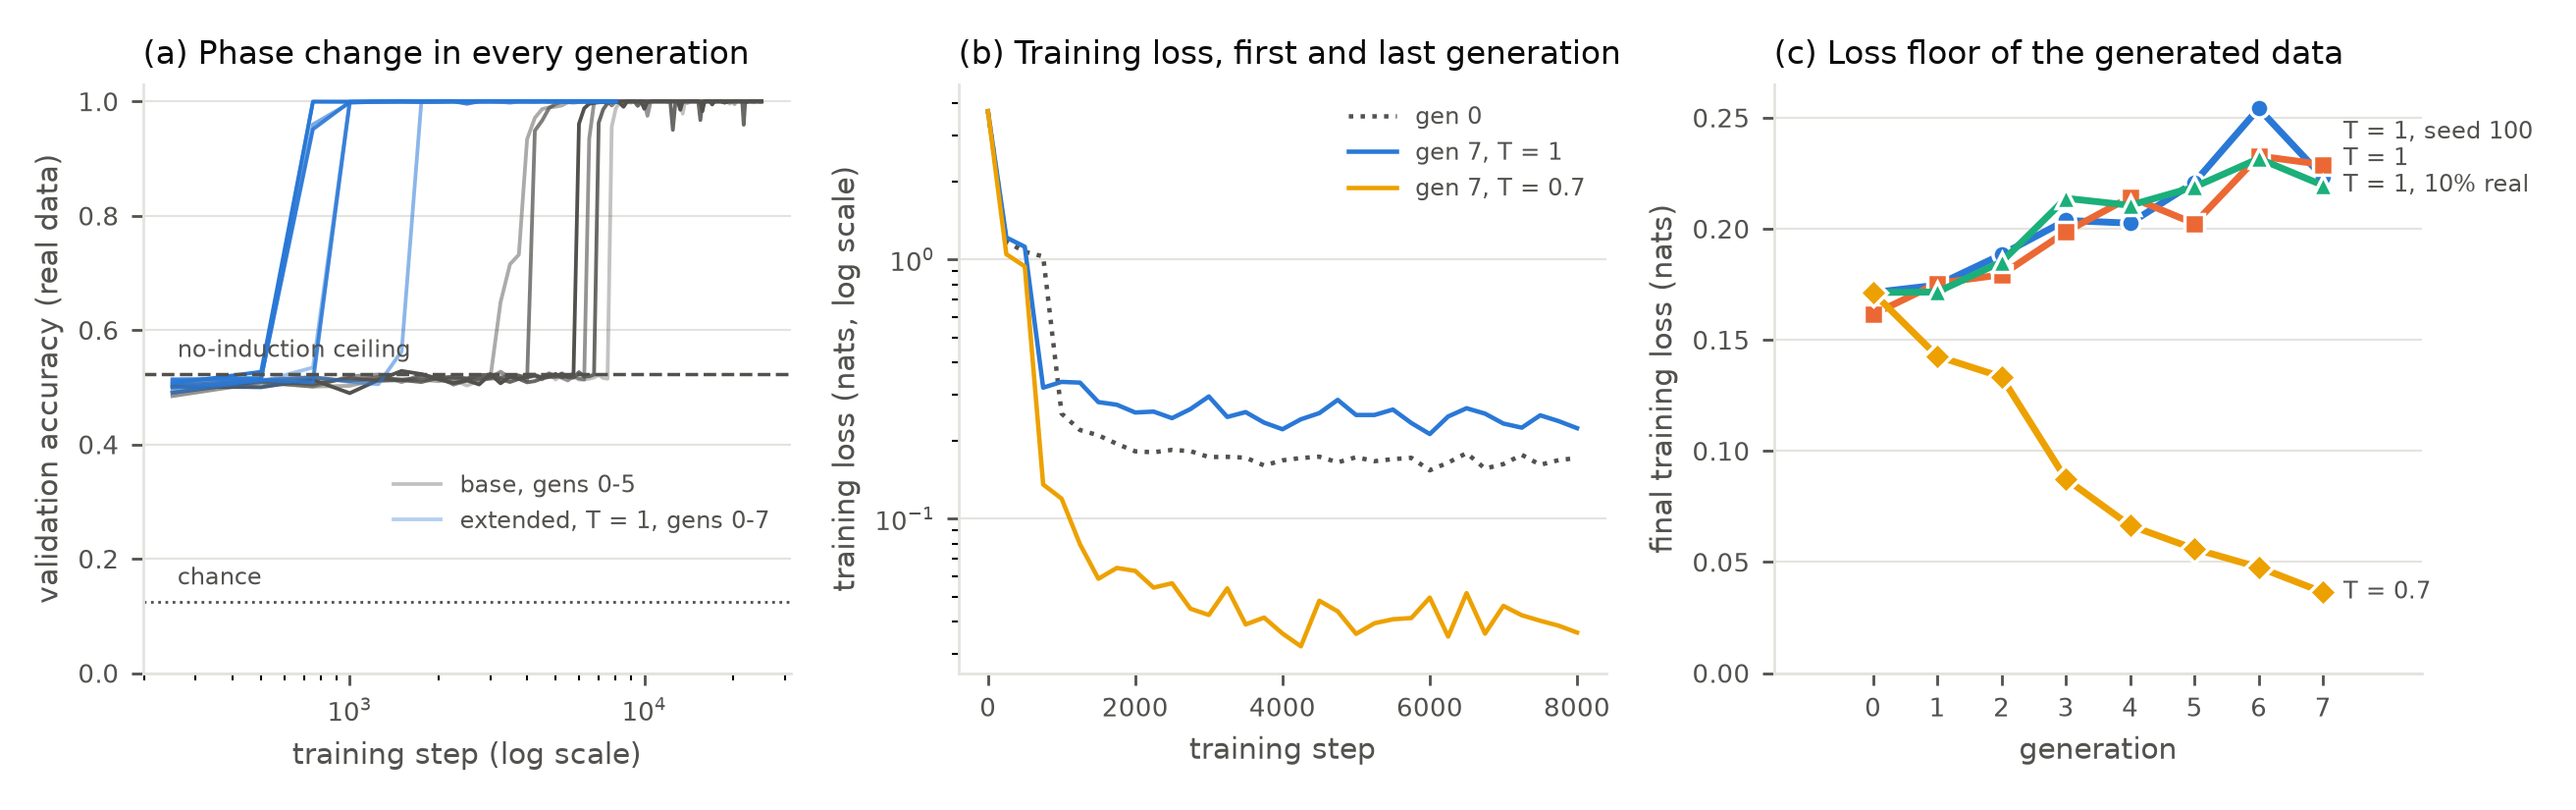
\includegraphics[width=0.94\textwidth]{images/fig_training.png}
  \caption{\looseness=-1 Training dynamics. (a) Validation accuracy (query label, real data) during training for every generation of the base chain (grey) and the seed-0 $T=1$ extended chain (blue; darker means later generation). Every model sits at the 0.523 no-induction ceiling until a sudden phase change; extended models cross it about seven times sooner (median 875 vs.\ 6{,}250 steps). (b) Training loss of generations 0 and 7. Its floor comes from the free next-symbol choice and moves in opposite directions at $T=1$ and $T=0.7$. (c) Final training loss of each generation: synthetic data becomes harder to predict at $T=1$ and easier at $T=0.7$, since sharpened choices are more predictable.}
  \label{fig:training}
\end{figure}

\begin{table}[H]
\centering
\caption{\looseness=-1 Next-symbol choice on held-out real data for the first chains (the added chains are in Table~\ref{tab:revision}). leak., mis.: leakage and misallocation in nats (Eq.~\ref{eq:split}); 1-slot: choice probability of a symbol filling one slot (true 0.125).}
\small
\begin{tabular}{@{}lccccc@{}}
\toprule
Chain (generation) & leak. & mis. & KL & slope & 1-slot \\
\midrule
$T{=}1$, seed 0 (0) & 0.023 & 0.076 & 0.099 & 1.01 & 0.118 \\
$T{=}1$, seed 0 (7) & 0.161 & 0.398 & 0.558 & 1.27 & 0.085 \\
$T{=}1$, seed 100 (7) & 0.163 & 0.387 & 0.550 & 1.04 & 0.118 \\
$T{=}1$, 10\% real (7) & 0.125 & 0.171 & 0.296 & 1.14 & 0.103 \\
$T{=}0.7$ (7) & 0.005 & 2.562 & 2.567 & 1.92 & 0.017 \\
\bottomrule
\end{tabular}
\label{tab:collapse}
\end{table}

\begin{table}[H]
\centering
\caption{\looseness=-1 Accuracy on each model's own training data (train) against the share of training rows whose label agrees with the context (data ok) and accuracy on held-out real data (real), for the first and last generation of each chain. Next-label ``data ok'' counts only rows whose next symbol is in the context. From generation 1 the training labels were sampled by the previous model, so train accuracy is measured against those samples, errors included. Train next-label accuracy falls to 0.91 at $T{=}1$ while real next-label accuracy stays $\geq$0.997: the errors are in the synthetic data, and the model does not reproduce them on real contexts. Made by \texttt{scripts/train\_accuracy.py}.}
\small
\begin{tabular}{@{}lccccccc@{}}
\toprule
& \multicolumn{3}{c}{Query label} & \multicolumn{3}{c}{Next label} & \\
\cmidrule(lr){2-4}\cmidrule(lr){5-7}
Chain (generation) & train & data ok & real & train & data ok & real & Train loss \\
\midrule
Base (0) & 1.0000 & 1.0000 & 1.0000 & -- & -- & -- & 0.0000 \\
Base (5) & 1.0000 & 1.0000 & 1.0000 & -- & -- & -- & 0.0000 \\
$T{=}1$, seed 0 (0) & 0.9998 & 1.0000 & 0.9996 & 0.9994 & 1.0000 & 0.9995 & 0.166 \\
$T{=}1$, seed 0 (7) & 0.9993 & 0.9993 & 1.0000 & 0.9076 & 0.9949 & 0.9988 & 0.244 \\
$T{=}1$, seed 100 (0) & 1.0000 & 1.0000 & 1.0000 & 1.0000 & 1.0000 & 1.0000 & 0.165 \\
$T{=}1$, seed 100 (7) & 0.9976 & 0.9976 & 1.0000 & 0.9088 & 0.9936 & 0.9998 & 0.247 \\
$T{=}1$, 10\% real (7) & 0.9982 & 0.9993 & 0.9993 & 0.9276 & 0.9950 & 0.9973 & 0.245 \\
$T{=}0.7$ (7) & 0.9997 & 0.9999 & 0.9998 & 0.9994 & 1.0000 & 0.9996 & 0.039 \\
\bottomrule
\end{tabular}
\label{tab:train}
\end{table}

\begin{table}[H]
\centering
\caption{\looseness=-1 Fit of $x_g = (1-\alpha)\,x_{g-1} + \delta$ over generations 0--7 on held-out real data, for leakage and misallocation (both in nats; Eq.~\ref{eq:split}). Derivation: if each model reproduces the leakage of its training data and adds a fresh error $\delta$, and a share $r$ of the training rows is real (with $p_\text{out}{=}0$), then $p_{\text{out},g} = (1-r)\,p_{\text{out},g-1} + \delta$, so $\alpha \approx r$ (to first order also for leakage in nats, which is close to $p_\text{out}$ when small); for $\alpha > 0$, $x$ settles at $\delta/\alpha$. Without real data $\alpha \approx 0$ and leakage grows by $\delta$ per generation. With 10\% real data the fitted leakage $\alpha$ (0.12 and 0.06 in two seeds) is close to $r{=}0.1$. Negative $\alpha$ means accelerating growth. Eight near-linear points give a high $R^2$ almost regardless of the model, so these fits describe the trajectories rather than test the recursion; the misallocation $\alpha$ changes sign between the two $T{=}1$ seeds, and its 10\%-real fit is weak. Made by \texttt{scripts/leakage\_fit.py}.}
\small
\begin{tabular}{@{}lcccccc@{}}
\toprule
& \multicolumn{3}{c}{Leakage} & \multicolumn{3}{c}{Misallocation} \\
\cmidrule(lr){2-4}\cmidrule(lr){5-7}
Chain & $\alpha$ & $\delta$ & $R^2$ & $\alpha$ & $\delta$ & $R^2$ \\
\midrule
$T{=}1$, seed 0 & 0.033 & 0.023 & 0.991 & $-0.064$ & 0.033 & 0.986 \\
$T{=}1$, seed 100 & $-0.014$ & 0.020 & 0.993 & 0.091 & 0.064 & 0.984 \\
$T{=}1$, 10\% real & 0.124 & 0.024 & 0.998 & 0.317 & 0.057 & 0.833 \\
$T{=}1$, 10\% real, seed 100 & 0.058 & 0.018 & 0.992 & 0.412 & 0.076 & 0.801 \\
$T{=}0.7$ & 0.055 & $-0.002$ & 0.869 & $-0.137$ & 0.232 & 0.984 \\
$T{=}0.7$, seed 100 & 0.038 & $-0.001$ & 0.776 & $-0.094$ & 0.278 & 0.983 \\
$T{=}1$, 25{,}000 steps & $-0.006$ & 0.009 & 0.999 & 0.007 & 0.070 & 0.987 \\
$T{=}1$, generated contexts & $-0.140$ & 0.007 & 0.983 & 0.143 & 0.029 & 0.985 \\
$T{=}1$, accumulated data & 0.290 & 0.018 & 0.902 & 0.591 & 0.038 & 0.136 \\
\bottomrule
\end{tabular}
\label{tab:fit}
\end{table}

\begin{table}[H]
\centering
\caption{\looseness=-1 The seed-0 $T{=}0.7$ chain against a null model of pure sampling, on held-out real data (misallocation and leakage in nats). If every generation fitted its training data exactly, sampling at $T$ would give $p_g \propto p_0^{(1/T)^g}$. \emph{Pure}: $p_0{=}q$, the true choice. \emph{Anchored}: $p_0$ is the generation-0 model, errors included. Through generation 4 the trained chain tracks the anchored null closely in misallocation, slope and one-slot probability; from generation 5 it collapses less than the null, and it keeps some leakage, which the null removes within two generations. The seed-100 chain runs 10--40\% above its null in misallocation through generation 4 (1.30 vs.\ 1.18 at generation 4), then falls well below it (2.69 vs.\ 5.01 at generation 7; slope 1.77 vs.\ 1.95; one-slot 0.027 vs.\ 0.013). At $T{=}1$ both nulls are flat, so all $T{=}1$ drift is learner error. Made by \texttt{scripts/sampling\_null.py}.}
\small
\begin{tabular}{@{}lccccccccc@{}}
\toprule
& & Pure & \multicolumn{2}{c}{Misallocation} & \multicolumn{2}{c}{Leakage} & \multicolumn{2}{c}{Slope} & 1-slot (true 0.125) \\
\cmidrule(lr){3-3}\cmidrule(lr){4-5}\cmidrule(lr){6-7}\cmidrule(lr){8-9}\cmidrule(lr){10-10}
Gen. & $(1/T)^g$ & mis. & null & trained & null & trained & null & trained & null / trained \\
\midrule
0 & 1.00 & 0.000 & 0.076 & 0.076 & 0.023 & 0.023 & 1.01 & 1.01 & 0.118 / 0.118 \\
1 & 1.43 & 0.016 & 0.161 & 0.174 & 0.004 & 0.025 & 1.26 & 1.30 & 0.085 / 0.079 \\
2 & 2.04 & 0.084 & 0.339 & 0.382 & 0.000 & 0.019 & 1.49 & 1.55 & 0.056 / 0.051 \\
3 & 2.92 & 0.243 & 0.662 & 0.697 & 0.000 & 0.016 & 1.68 & 1.73 & 0.035 / 0.032 \\
4 & 4.16 & 0.543 & 1.194 & 1.139 & 0.000 & 0.011 & 1.82 & 1.84 & 0.023 / 0.023 \\
5 & 5.95 & 1.044 & 2.018 & 1.679 & 0.000 & 0.008 & 1.90 & 1.90 & 0.016 / 0.019 \\
6 & 8.50 & 1.821 & 3.248 & 2.170 & 0.000 & 0.006 & 1.94 & 1.92 & 0.013 / 0.017 \\
7 & 12.14 & 2.979 & 5.045 & 2.562 & 0.000 & 0.005 & 1.96 & 1.92 & 0.011 / 0.017 \\
\bottomrule
\end{tabular}
\label{tab:null}
\end{table}

\begin{table}[H]
\centering
\caption{\looseness=-1 The same interventions scored on the query label (accuracy) and on the next-symbol choice (leakage and misallocation, nats; Eq.~\ref{eq:split}), on the same 10{,}000 held-out real sequences. Medians [range] over the 72 extended models (a generation-0 model shared by several chains is counted in each). \emph{Induction head}: the layer-1 head whose resampling most lowers query accuracy; \emph{previous-token head}: the same in layer 0, patched only into layer 1's queries, keys or values, including the route via the layer-0 MLP. The key path that carries the previous-token head's effect on the query label leaves the choice unchanged (at most 0.07 nats in the 64 models with real contexts; at most 0.19, mainly via values, in the generated-context chain), and the induction head matters no more for the choice than the layer-1 heads that do not matter for the query. Across all 78 models the best previous-token score is 0.89--1.00 and the best induction score 0.96--1.00 (attention from each label to its symbol, and from the query to the label after its earlier occurrence, on the same sequences; \texttt{scripts/attention\_scores.py}). In 8 models (the seed-100 generation-0 model, shared by three chains; $T{=}0.7$ generations 1 and 4; 10\%-real generations 4 and 6; accumulated-data generation 4) no single layer-0 head drops query accuracy below 0.9, yet resampling all of layer 0 gives 0.37--0.42: several heads share the previous-token role, so these are left out of the path shares. Made by \texttt{scripts/choice\_circuit.py}.}
\small
\begin{tabular}{@{}lccc@{}}
\toprule
Resampled & Query accuracy & Choice leakage & Choice misallocation \\
\midrule
nothing & 1.00 [1.00, 1.00] & 0.05 [0.01, 0.16] & 0.17 [0.03, 2.69] \\
all of layer 0 & 0.38 [0.20, 0.42] & 1.31 [0.52, 2.18] & 1.70 [0.96, 5.17] \\
all of layer 1 & 0.13 [0.13, 0.14] & 0.52 [0.09, 1.05] & 1.33 [0.38, 3.32] \\
induction head & 0.54 [0.13, 0.97] & 0.09 [0.01, 0.25] & 0.40 [0.08, 2.59] \\
other layer-1 heads (mean) & 0.99 [0.90, 1.00] & 0.10 [0.01, 0.24] & 0.40 [0.16, 2.81] \\
previous-token head $\to$ queries & 1.00 [1.00, 1.00] & 0.05 [0.01, 0.17] & 0.18 [0.03, 2.67] \\
previous-token head $\to$ keys & 0.59 [0.40, 0.98] & 0.05 [0.01, 0.17] & 0.18 [0.04, 2.69] \\
previous-token head $\to$ values & 1.00 [0.93, 1.00] & 0.05 [0.01, 0.16] & 0.19 [0.06, 2.68] \\
\bottomrule
\end{tabular}
\label{tab:choice}
\end{table}

\begin{table}[H]
\centering
\caption{\looseness=-1 Chains added after review: next-symbol choice on held-out real data at generations 0 and 7 (as in Table~\ref{tab:collapse}), and real-data query accuracy. \emph{25{,}000 steps}: the seed-0 $T{=}1$ chain with each generation trained 3$\times$ longer on the same data; compare Table~\ref{tab:collapse} (8{,}000 steps: leakage 0.023 and misallocation 0.076 nats at generation 0, 0.161 and 0.398 at generation 7). \emph{Generated contexts}: the model writes the whole sequence, with a loss on every token. Its contexts at generation 0 $\to$ 7: repeated symbols keep their label 99.9\% $\to$ 99.5\%; distinct symbols per context 3.66 $\to$ 4.12 (real 3.60, at most 4); query in the context 99.2\% $\to$ 91.7\%; generated query label agrees with the context 99.4\% $\to$ 92.2\%; exact KL of the context symbols 0.18 $\to$ 1.17 nats per sequence. \emph{Accumulated data}: each generation trains on the real data plus all earlier generations' data \citep{gerstgrasser2024inevitable}. Made by \texttt{scripts/cluster/revision.sbatch} and \texttt{revision\_analysis.sbatch}.}
\small
\begin{tabular}{@{}lcccccc@{}}
\toprule
Chain (generation) & leak. & mis. & KL & slope & 1-slot & query acc. \\
\midrule
25{,}000 steps (0) & 0.010 & 0.102 & 0.112 & 1.03 & 0.115 & 1.0000 \\
25{,}000 steps (7) & 0.074 & 0.578 & 0.652 & 1.11 & 0.100 & 0.9999 \\
Generated contexts (0) & 0.007 & 0.031 & 0.038 & 0.94 & 0.128 & 0.9999 \\
Generated contexts (7) & 0.096 & 0.145 & 0.241 & 0.89 & 0.120 & 0.9999 \\
Accumulated data (7) & 0.059 & 0.068 & 0.127 & 1.08 & 0.112 & 0.9999 \\
$T{=}0.7$, seed 100 (7) & 0.005 & 2.690 & 2.695 & 1.77 & 0.027 & 0.9989 \\
10\% real, seed 100 (7) & 0.115 & 0.191 & 0.305 & 1.04 & 0.116 & 1.0000 \\
\bottomrule
\end{tabular}
\label{tab:revision}
\end{table}

\begin{figure}[H]
  \centering
  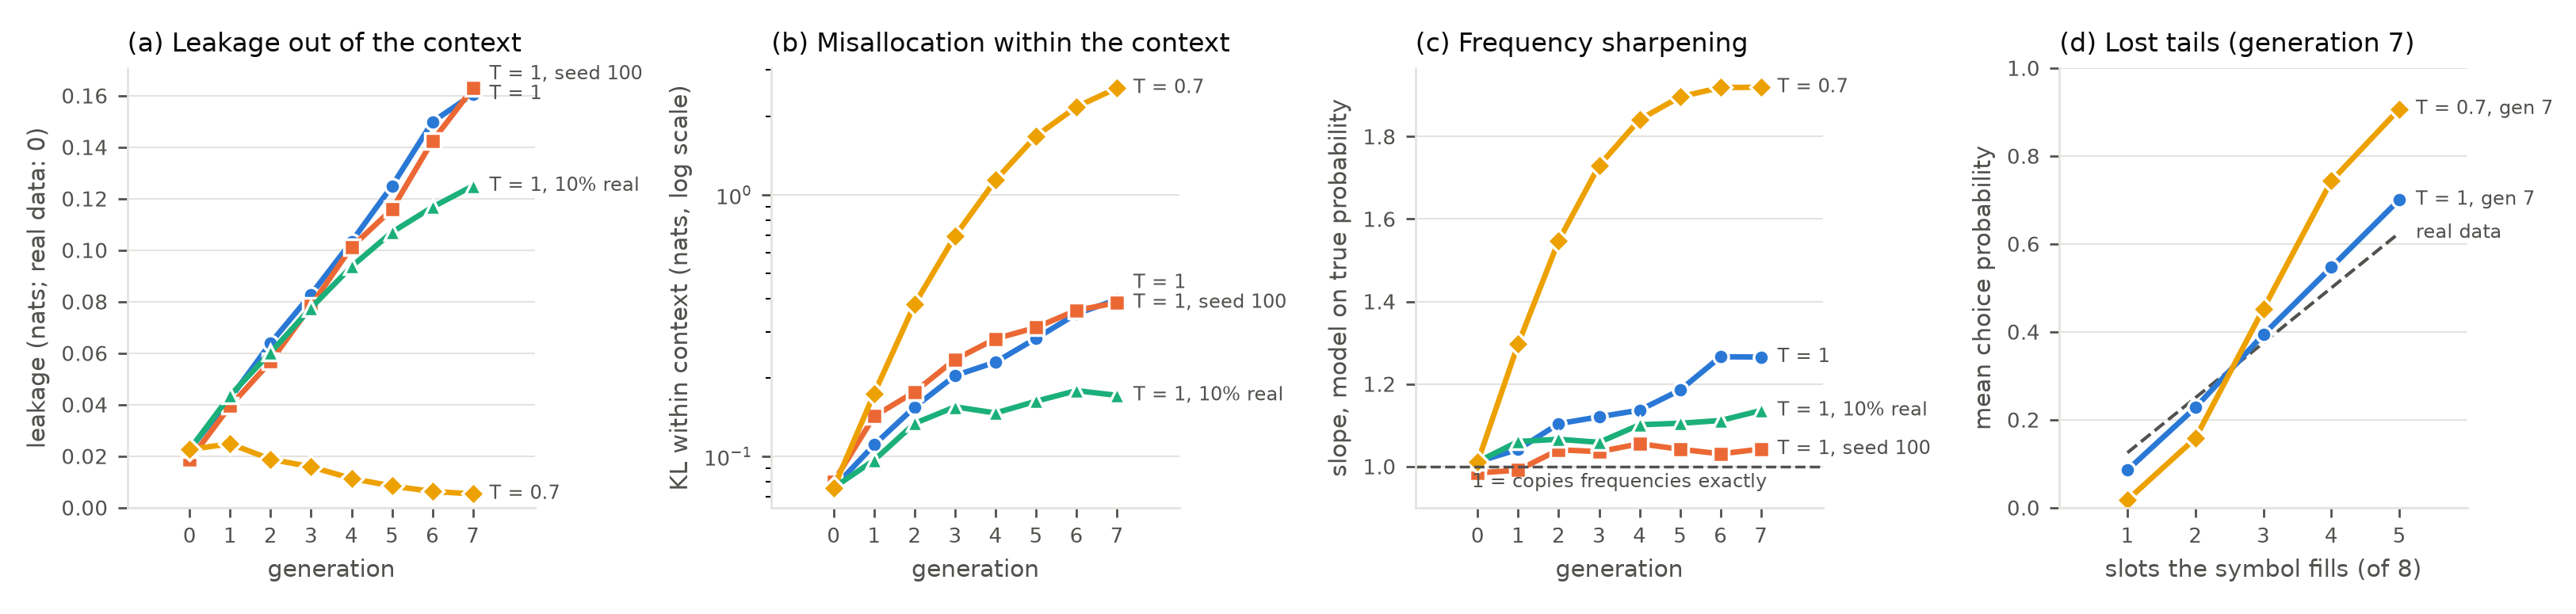
\includegraphics[width=\textwidth]{images/fig_collapse.png}
  \caption{\looseness=-1 Drift of the next-symbol choice on held-out real data. (a) Leakage rises linearly at $T{=}1$ and falls at $T{=}0.7$. (b) Misallocation rises in every chain (log scale); 10\% real data caps it. (c) Sharpening: strong at $T{=}0.7$, seed-dependent at $T{=}1$. (d) Choice probability by how many slots a symbol fills at generation 7: single-slot symbols almost vanish at $T{=}0.7$.}
  \label{fig:collapse}
\end{figure}

\begin{figure}[H]
  \centering
  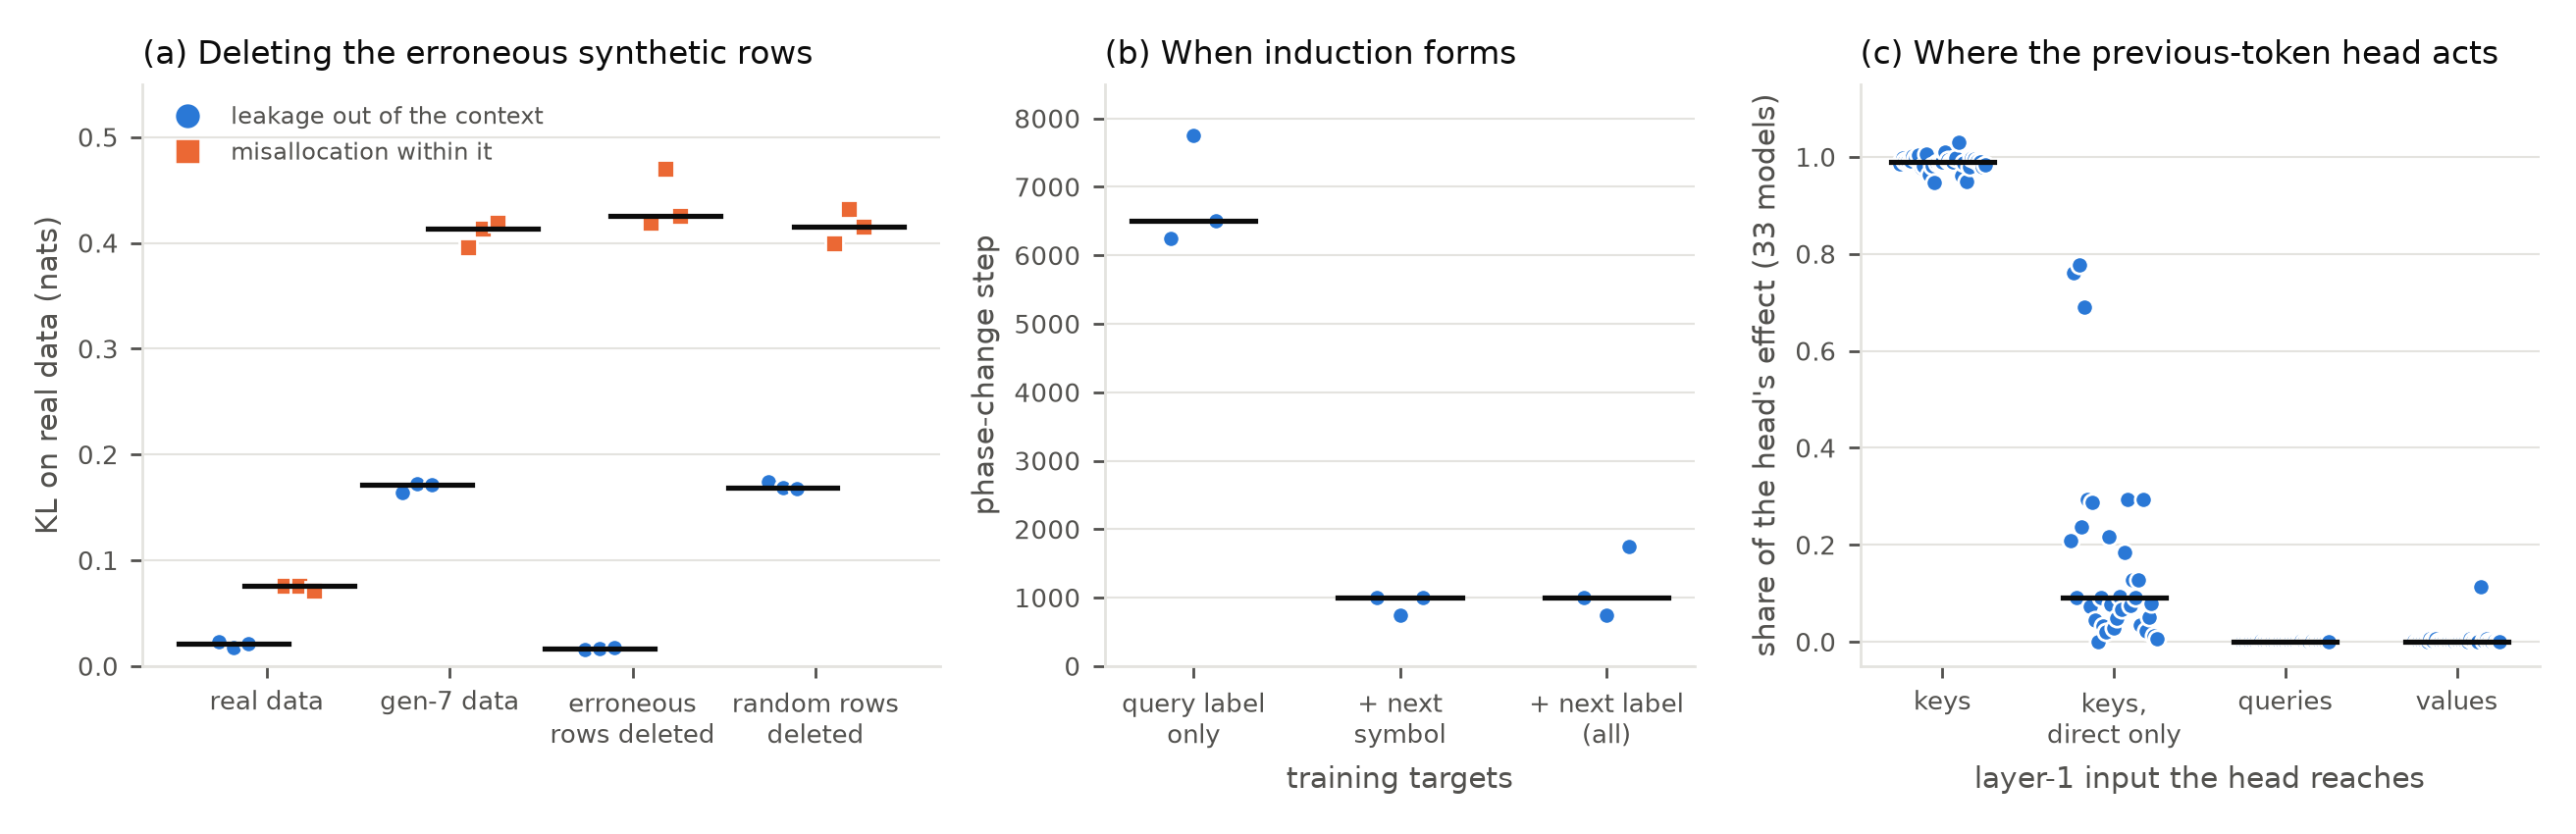
\includegraphics[width=0.8\textwidth]{images/fig_interventions.png}
  \caption{\looseness=-1 Interventions (dots: seeds or models; bars: medians). (a) Deleting generation-7's contradicting rows restores leakage (blue) but not misallocation (orange); deleting random rows does neither. (b) The next-symbol target makes induction form seven times sooner. (c) Share of the previous-token head's effect carried by each path into layer 1 (33 models): nearly all goes to the keys, mostly via the layer-0 MLP.}
  \label{fig:interventions}
\end{figure}

\IfFileExists{images/fig_embeddings.png}{
\begin{figure}[H]
  \centering
  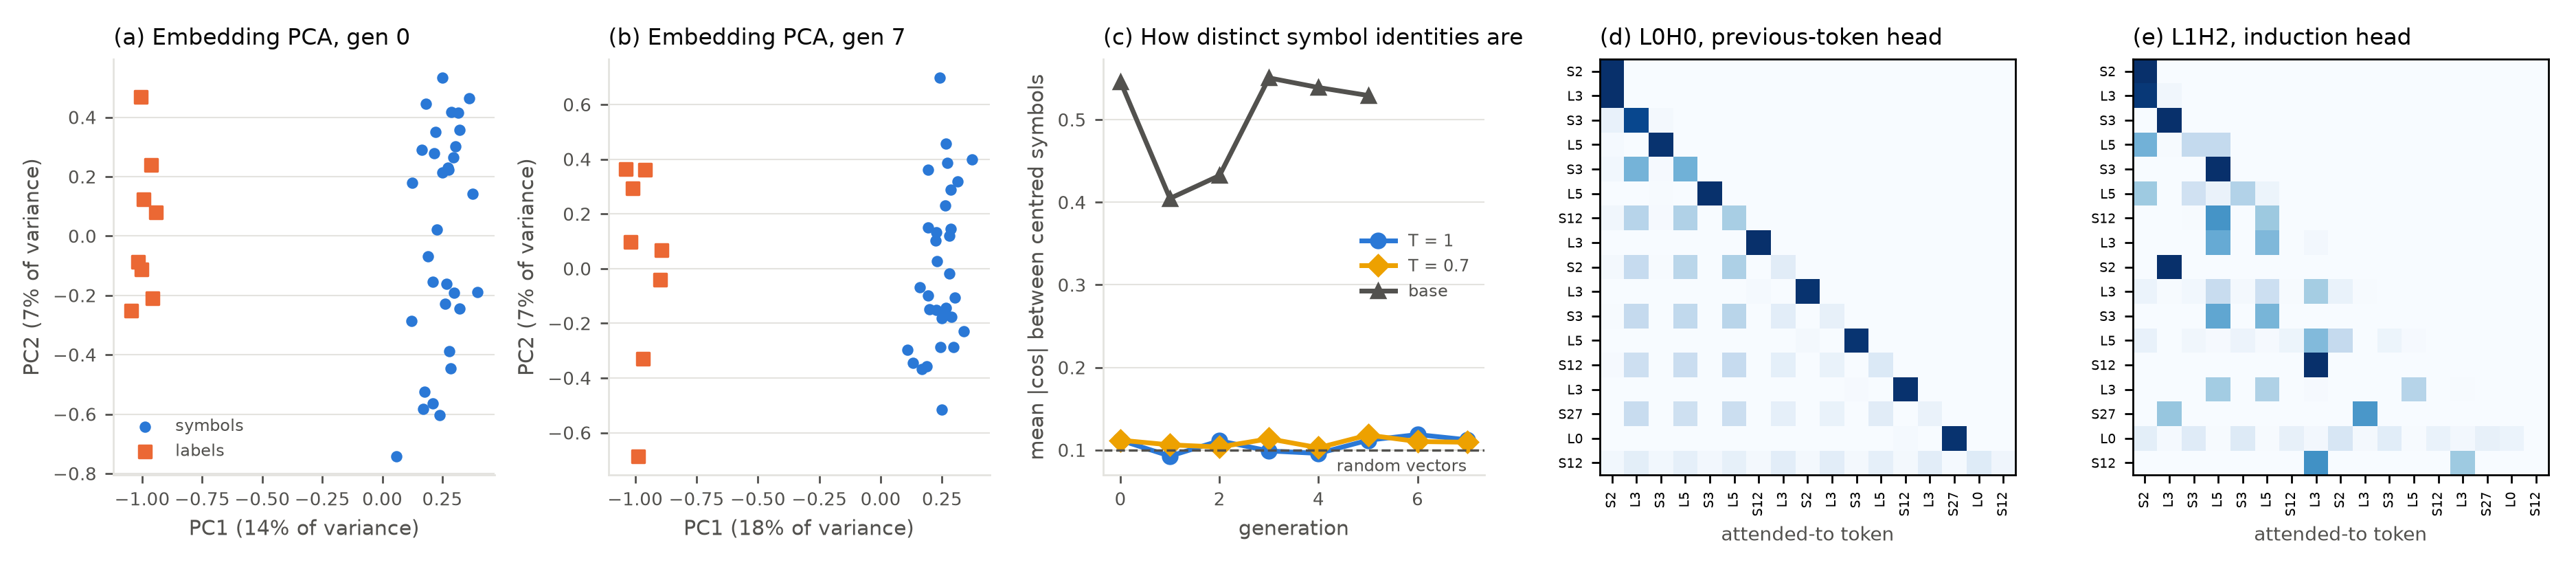
\includegraphics[width=0.98\textwidth]{images/fig_embeddings.png}
  \caption{\looseness=-1 Token embeddings and attention. (a, b) PCA of the symbol and label embeddings at generations 0 and 7 of the seed-0 $T=1$ chain: symbols and labels stay in two separate clusters. (c) Mean $|\cos|$ between symbol embeddings after removing the mean symbol. Extended models keep symbols as distinct as random vectors (0.09--0.12; dashed line 0.10) in every generation of both chains, and symbols that the synthetic data over-chooses do not gain larger embedding norms (correlation $-0.46$ to $+0.29$, changing sign between generations). Base models keep them far less distinct (0.40--0.55), plausibly because they never have to output a symbol through the tied unembedding. (d, e) Attention of the generation-7 model on one real sequence. The previous-token head (L0H0) sends each label to the symbol before it; the induction head (L1H2) sends each repeated symbol to the label that followed its earlier occurrence. Collapse leaves both the embedding and the attention pattern intact.}
  \label{fig:embeddings}
\end{figure}
}{}

\end{document}
